\documentclass[tikz,border=7pt]{standalone}
\begin{document}
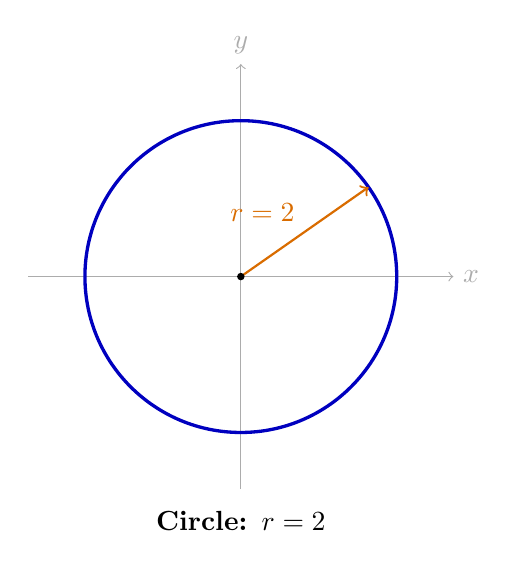
\begin{tikzpicture}[scale=.9]
\draw[->,gray!65] (-3,0)--(3,0) node[right] {$x$};
\draw[->,gray!65] (0,-3)--(0,3) node[above] {$y$};
\draw[blue!75!black,very thick] (0,0) circle (2.2);
\draw[->,orange!85!black,thick] (0,0)--(35:2.2) node[midway,above left] {$r=2$};
\fill (0,0) circle (1.5pt);
\node[font=\bfseries] at (0,-3.45) {Circle: $r=2$};
\end{tikzpicture}
\end{document}
